%% template.tex
%% from
%% bare_conf.tex
%% V1.4b
%% 2015/08/26
%% by Michael Shell
%% See:
%% http://www.michaelshell.org/
%% for current contact information.
%%
%% This is a skeleton file demonstrating the use of IEEEtran.cls
%% (requires IEEEtran.cls version 1.8b or later) with an IEEE
%% conference paper.
%%
%% Support sites:
%% http://www.michaelshell.org/tex/ieeetran/
%% http://www.ctan.org/pkg/ieeetran
%% and
%% http://www.ieee.org/

%%*************************************************************************
%% Legal Notice:
%% This code is offered as-is without any warranty either expressed or
%% implied; without even the implied warranty of MERCHANTABILITY or
%% FITNESS FOR A PARTICULAR PURPOSE!
%% User assumes all risk.
%% In no event shall the IEEE or any contributor to this code be liable for
%% any damages or losses, including, but not limited to, incidental,
%% consequential, or any other damages, resulting from the use or misuse
%% of any information contained here.
%%
%% All comments are the opinions of their respective authors and are not
%% necessarily endorsed by the IEEE.
%%
%% This work is distributed under the LaTeX Project Public License (LPPL)
%% ( http://www.latex-project.org/ ) version 1.3, and may be freely used,
%% distributed and modified. A copy of the LPPL, version 1.3, is included
%% in the base LaTeX documentation of all distributions of LaTeX released
%% 2003/12/01 or later.
%% Retain all contribution notices and credits.
%% ** Modified files should be clearly indicated as such, including  **
%% ** renaming them and changing author support contact information. **
%%*************************************************************************


% *** Authors should verify (and, if needed, correct) their LaTeX system  ***
% *** with the testflow diagnostic prior to trusting their LaTeX platform ***
% *** with production work. The IEEE's font choices and paper sizes can   ***
% *** trigger bugs that do not appear when using other class files.       ***                          ***
% The testflow support page is at:
% http://www.michaelshell.org/tex/testflow/

\documentclass[conference,final,]{IEEEtran}
% Some Computer Society conferences also require the compsoc mode option,
% but others use the standard conference format.
%
% If IEEEtran.cls has not been installed into the LaTeX system files,
% manually specify the path to it like:
% \documentclass[conference]{../sty/IEEEtran}





% Some very useful LaTeX packages include:
% (uncomment the ones you want to load)


% *** MISC UTILITY PACKAGES ***
%
%\usepackage{ifpdf}
% Heiko Oberdiek's ifpdf.sty is very useful if you need conditional
% compilation based on whether the output is pdf or dvi.
% usage:
% \ifpdf
%   % pdf code
% \else
%   % dvi code
% \fi
% The latest version of ifpdf.sty can be obtained from:
% http://www.ctan.org/pkg/ifpdf
% Also, note that IEEEtran.cls V1.7 and later provides a builtin
% \ifCLASSINFOpdf conditional that works the same way.
% When switching from latex to pdflatex and vice-versa, the compiler may
% have to be run twice to clear warning/error messages.






% *** CITATION PACKAGES ***
%
%\usepackage{cite}
% cite.sty was written by Donald Arseneau
% V1.6 and later of IEEEtran pre-defines the format of the cite.sty package
% \cite{} output to follow that of the IEEE. Loading the cite package will
% result in citation numbers being automatically sorted and properly
% "compressed/ranged". e.g., [1], [9], [2], [7], [5], [6] without using
% cite.sty will become [1], [2], [5]--[7], [9] using cite.sty. cite.sty's
% \cite will automatically add leading space, if needed. Use cite.sty's
% noadjust option (cite.sty V3.8 and later) if you want to turn this off
% such as if a citation ever needs to be enclosed in parenthesis.
% cite.sty is already installed on most LaTeX systems. Be sure and use
% version 5.0 (2009-03-20) and later if using hyperref.sty.
% The latest version can be obtained at:
% http://www.ctan.org/pkg/cite
% The documentation is contained in the cite.sty file itself.






% *** GRAPHICS RELATED PACKAGES ***
%
\ifCLASSINFOpdf
  % \usepackage[pdftex]{graphicx}
  % declare the path(s) where your graphic files are
  % \graphicspath{{../pdf/}{../jpeg/}}
  % and their extensions so you won't have to specify these with
  % every instance of \includegraphics
  % \DeclareGraphicsExtensions{.pdf,.jpeg,.png}
\else
  % or other class option (dvipsone, dvipdf, if not using dvips). graphicx
  % will default to the driver specified in the system graphics.cfg if no
  % driver is specified.
  % \usepackage[dvips]{graphicx}
  % declare the path(s) where your graphic files are
  % \graphicspath{{../eps/}}
  % and their extensions so you won't have to specify these with
  % every instance of \includegraphics
  % \DeclareGraphicsExtensions{.eps}
\fi
% graphicx was written by David Carlisle and Sebastian Rahtz. It is
% required if you want graphics, photos, etc. graphicx.sty is already
% installed on most LaTeX systems. The latest version and documentation
% can be obtained at:
% http://www.ctan.org/pkg/graphicx
% Another good source of documentation is "Using Imported Graphics in
% LaTeX2e" by Keith Reckdahl which can be found at:
% http://www.ctan.org/pkg/epslatex
%
% latex, and pdflatex in dvi mode, support graphics in encapsulated
% postscript (.eps) format. pdflatex in pdf mode supports graphics
% in .pdf, .jpeg, .png and .mps (metapost) formats. Users should ensure
% that all non-photo figures use a vector format (.eps, .pdf, .mps) and
% not a bitmapped formats (.jpeg, .png). The IEEE frowns on bitmapped formats
% which can result in "jaggedy"/blurry rendering of lines and letters as
% well as large increases in file sizes.
%
% You can find documentation about the pdfTeX application at:
% http://www.tug.org/applications/pdftex





% *** MATH PACKAGES ***
%
%\usepackage{amsmath}
% A popular package from the American Mathematical Society that provides
% many useful and powerful commands for dealing with mathematics.
%
% Note that the amsmath package sets \interdisplaylinepenalty to 10000
% thus preventing page breaks from occurring within multiline equations. Use:
%\interdisplaylinepenalty=2500
% after loading amsmath to restore such page breaks as IEEEtran.cls normally
% does. amsmath.sty is already installed on most LaTeX systems. The latest
% version and documentation can be obtained at:
% http://www.ctan.org/pkg/amsmath





% *** SPECIALIZED LIST PACKAGES ***
%
%\usepackage{algorithmic}
% algorithmic.sty was written by Peter Williams and Rogerio Brito.
% This package provides an algorithmic environment fo describing algorithms.
% You can use the algorithmic environment in-text or within a figure
% environment to provide for a floating algorithm. Do NOT use the algorithm
% floating environment provided by algorithm.sty (by the same authors) or
% algorithm2e.sty (by Christophe Fiorio) as the IEEE does not use dedicated
% algorithm float types and packages that provide these will not provide
% correct IEEE style captions. The latest version and documentation of
% algorithmic.sty can be obtained at:
% http://www.ctan.org/pkg/algorithms
% Also of interest may be the (relatively newer and more customizable)
% algorithmicx.sty package by Szasz Janos:
% http://www.ctan.org/pkg/algorithmicx




% *** ALIGNMENT PACKAGES ***
%
%\usepackage{array}
% Frank Mittelbach's and David Carlisle's array.sty patches and improves
% the standard LaTeX2e array and tabular environments to provide better
% appearance and additional user controls. As the default LaTeX2e table
% generation code is lacking to the point of almost being broken with
% respect to the quality of the end results, all users are strongly
% advised to use an enhanced (at the very least that provided by array.sty)
% set of table tools. array.sty is already installed on most systems. The
% latest version and documentation can be obtained at:
% http://www.ctan.org/pkg/array


% IEEEtran contains the IEEEeqnarray family of commands that can be used to
% generate multiline equations as well as matrices, tables, etc., of high
% quality.




% *** SUBFIGURE PACKAGES ***
%\ifCLASSOPTIONcompsoc
%  \usepackage[caption=false,font=normalsize,labelfont=sf,textfont=sf]{subfig}
%\else
%  \usepackage[caption=false,font=footnotesize]{subfig}
%\fi
% subfig.sty, written by Steven Douglas Cochran, is the modern replacement
% for subfigure.sty, the latter of which is no longer maintained and is
% incompatible with some LaTeX packages including fixltx2e. However,
% subfig.sty requires and automatically loads Axel Sommerfeldt's caption.sty
% which will override IEEEtran.cls' handling of captions and this will result
% in non-IEEE style figure/table captions. To prevent this problem, be sure
% and invoke subfig.sty's "caption=false" package option (available since
% subfig.sty version 1.3, 2005/06/28) as this is will preserve IEEEtran.cls
% handling of captions.
% Note that the Computer Society format requires a larger sans serif font
% than the serif footnote size font used in traditional IEEE formatting
% and thus the need to invoke different subfig.sty package options depending
% on whether compsoc mode has been enabled.
%
% The latest version and documentation of subfig.sty can be obtained at:
% http://www.ctan.org/pkg/subfig




% *** FLOAT PACKAGES ***
%

%\usepackage{fixltx2e}
% fixltx2e, the successor to the earlier fix2col.sty, was written by
% Frank Mittelbach and David Carlisle. This package corrects a few problems
% in the LaTeX2e kernel, the most notable of which is that in current
% LaTeX2e releases, the ordering of single and double column floats is not
% guaranteed to be preserved. Thus, an unpatched LaTeX2e can allow a
% single column figure to be placed prior to an earlier double column
% figure.
% Be aware that LaTeX2e kernels dated 2015 and later have fixltx2e.sty's
% corrections already built into the system in which case a warning will
% be issued if an attempt is made to load fixltx2e.sty as it is no longer
% needed.
% The latest version and documentation can be found at:
% http://www.ctan.org/pkg/fixltx2e


%\usepackage{stfloats}
% stfloats.sty was written by Sigitas Tolusis. This package gives LaTeX2e
% the ability to do double column floats at the bottom of the page as well
% as the top. (e.g., "\begin{figure*}[!b]" is not normally possible in
% LaTeX2e). It also provides a command:
%\fnbelowfloat
% to enable the placement of footnotes below bottom floats (the standard
% LaTeX2e kernel puts them above bottom floats). This is an invasive package
% which rewrites many portions of the LaTeX2e float routines. It may not work
% with other packages that modify the LaTeX2e float routines. The latest
% version and documentation can be obtained at:
% http://www.ctan.org/pkg/stfloats
% Do not use the stfloats baselinefloat ability as the IEEE does not allow
% \baselineskip to stretch. Authors submitting work to the IEEE should note
% that the IEEE rarely uses double column equations and that authors should try
% to avoid such use. Do not be tempted to use the cuted.sty or midfloat.sty
% packages (also by Sigitas Tolusis) as the IEEE does not format its papers in
% such ways.
% Do not attempt to use stfloats with fixltx2e as they are incompatible.
% Instead, use Morten Hogholm'a dblfloatfix which combines the features
% of both fixltx2e and stfloats:
%
% \usepackage{dblfloatfix}
% The latest version can be found at:
% http://www.ctan.org/pkg/dblfloatfix




% *** PDF, URL AND HYPERLINK PACKAGES ***
%
%\usepackage{url}
% url.sty was written by Donald Arseneau. It provides better support for
% handling and breaking URLs. url.sty is already installed on most LaTeX
% systems. The latest version and documentation can be obtained at:
% http://www.ctan.org/pkg/url
% Basically, \url{my_url_here}.




% *** Do not adjust lengths that control margins, column widths, etc. ***
% *** Do not use packages that alter fonts (such as pslatex).         ***
% There should be no need to do such things with IEEEtran.cls V1.6 and later.
% (Unless specifically asked to do so by the journal or conference you plan
% to submit to, of course. )



%% BEGIN MY ADDITIONS %%


\usepackage{graphicx}
% We will generate all images so they have a width \maxwidth. This means
% that they will get their normal width if they fit onto the page, but
% are scaled down if they would overflow the margins.
\makeatletter
\def\maxwidth{\ifdim\Gin@nat@width>\linewidth\linewidth
\else\Gin@nat@width\fi}
\makeatother
\let\Oldincludegraphics\includegraphics
\renewcommand{\includegraphics}[1]{\Oldincludegraphics[width=\maxwidth]{#1}}

\usepackage[unicode=true]{hyperref}

\hypersetup{
            pdftitle={Land doesn't get cancer, people do: an experiment comparing the effectiveness of two displays},
            pdfkeywords={statistics, visual inference, geospatial, population},
            pdfborder={0 0 0},
            breaklinks=true}
\urlstyle{same}  % don't use monospace font for urls

% Pandoc toggle for numbering sections (defaults to be off)
\setcounter{secnumdepth}{0}

% Pandoc syntax highlighting

% Pandoc header

\providecommand{\tightlist}{%
  \setlength{\itemsep}{0pt}\setlength{\parskip}{0pt}}

%% END MY ADDITIONS %%


\hyphenation{op-tical net-works semi-conduc-tor}

\begin{document}
%
% paper title
% Titles are generally capitalized except for words such as a, an, and, as,
% at, but, by, for, in, nor, of, on, or, the, to and up, which are usually
% not capitalized unless they are the first or last word of the title.
% Linebreaks \\ can be used within to get better formatting as desired.
% Do not put math or special symbols in the title.
\title{Land doesn't get cancer, people do: an experiment comparing the
effectiveness of two displays}

% author names and affiliations
% use a multiple column layout for up to three different
% affiliations

\author{

%% ---- classic IEEETrans wide authors' list ----------------
 % -- end affiliation.wide
%% ----------------------------------------------------------



%% ---- classic IEEETrans one column per institution --------
 %% -- end if/affiliation.institution-columnar
%% ----------------------------------------------------------





%% ---- one column per author, classic/default IEEETrans ----
 % -- beg affiliation.author-columnar
  %% -- beg for/affiliation.institution.author
\IEEEauthorblockN{
Stephanie Kobakian
}
\IEEEauthorblockA{Queensland University of Technology\\
Science and Engineering Faculty\\
Brisbane, Australia
\\stephanie.kobakian@qut.edu.au
}
 %% -- end for/affiliation.institution.author
\and
  %% -- beg for/affiliation.institution.author
\IEEEauthorblockN{
Dianne Cook
}
\IEEEauthorblockA{Monash University\\
Econometrics and Business Statistics Faculty\\
Melbourne, Australia
\\dicook@monash.edu
}
 %% -- end for/affiliation.institution.author
 %% -- end for/affiliation.institution
 %% -- end if/affiliation.institution-columnar
%% ----------------------------------------------------------

}

% conference papers do not typically use \thanks and this command
% is locked out in conference mode. If really needed, such as for
% the acknowledgment of grants, issue a \IEEEoverridecommandlockouts
% after \documentclass

% for over three affiliations, or if they all won't fit within the width
% of the page, use this alternative format:
%
%\author{\IEEEauthorblockN{Michael Shell\IEEEauthorrefmark{1},
%Homer Simpson\IEEEauthorrefmark{2},
%James Kirk\IEEEauthorrefmark{3},
%Montgomery Scott\IEEEauthorrefmark{3} and
%Eldon Tyrell\IEEEauthorrefmark{4}}
%\IEEEauthorblockA{\IEEEauthorrefmark{1}School of Electrical and Computer Engineering\\
%Georgia Institute of Technology,
%Atlanta, Georgia 30332--0250\\ Email: see http://www.michaelshell.org/contact.html}
%\IEEEauthorblockA{\IEEEauthorrefmark{2}Twentieth Century Fox, Springfield, USA\\
%Email: homer@thesimpsons.com}
%\IEEEauthorblockA{\IEEEauthorrefmark{3}Starfleet Academy, San Francisco, California 96678-2391\\
%Telephone: (800) 555--1212, Fax: (888) 555--1212}
%\IEEEauthorblockA{\IEEEauthorrefmark{4}Tyrell Inc., 123 Replicant Street, Los Angeles, California 90210--4321}}




% use for special paper notices
%\IEEEspecialpapernotice{(Invited Paper)}




% make the title area
\maketitle

% As a general rule, do not put math, special symbols or citations
% in the abstract
\begin{abstract}
The abstract goes here. On multiple lines eventually.
\end{abstract}

% keywords
\begin{IEEEkeywords}
statistics; visual inference; geospatial; population
\end{IEEEkeywords}

% use for special paper notices



% make the title area
\maketitle

% no keywords

% For peer review papers, you can put extra information on the cover
% page as needed:
% \ifCLASSOPTIONpeerreview
% \begin{center} \bfseries EDICS Category: 3-BBND \end{center}
% \fi
%
% For peerreview papers, this IEEEtran command inserts a page break and
% creates the second title. It will be ignored for other modes.
\IEEEpeerreviewmaketitle


\hypertarget{introduction}{%
\section{Introduction}\label{introduction}}

Geospatial statistics are often presented on the geographic map base. A
choropleth map is the common display to present aggreagated statistics
for geographic units, and they are often used to present statistics
regarding the population. Creating a choropleth map involves drawing the
administrative boundaries and filling them with colour to communicate
the value of the statistic. In Australia, there are sets of
administrative boundaries that define subdivisions of the population at
various granularities. The set of Australia statistical areas presents
an example of a heterogrenous distribution of area. The rural
communicates on a much larger geographic space than small inner city
communities. This has the negative effect of incorrectly showing the
spatial distribution of the statistic, especially when a spatial
distribution is related to the size of the areas, or the population
density.

An alternative display can also be used to effectively communicate a
spatial distribution for a set of heterogeneous areas. Viewers of
spatial distributions may come to incorrect conclusions.

\hypertarget{motivation}{%
\section{Motivation}\label{motivation}}

\hypertarget{australian-cancer-atlas}{%
\subsection{Australian Cancer Atlas}\label{australian-cancer-atlas}}

The Australian Cancer Atlas explores the burden of cancer on Australian
communities. There are many cancer types presented, and they can be
explored on an individual or aggregate level. The Australian communities
are examined at the Statistical Areas at Level 2 (SA2)(``Australian
Statistical Geography Standard (ASGS)''
\protect\hyperlink{ref-abs2016}{2018}) used by the Australian Bureau of
Statistics. Bayesian spatial smoothing has been applied to incorporate
the statistics of neighbouring areas, for both privacy and stability of
the estimates. The statistics that can be mapped are the diagnoses
(Standardised Incidence Rates) and excess deaths for each SA2,
communicated as the difference from the Australian average of the
statistics. The values of the statistic for each are communicated using
a diverging colour scheme.

The Australian Cancer Atlas communicates the trends in the distributions
of cancer over geographic space. It uses a choropleth map display and
diverging colour scheme to draw attention to relationships between
neighbouring areas.

\hypertarget{background}{%
\section{Background}\label{background}}

\hypertarget{methodology}{%
\subsection{Methodology}\label{methodology}}

Spatial visualisations - Choropleth However, the issue of using a
choropleth map base becomes obvious when considering the distributions.
Position is extremely important for analysis of a visualisation.

\hypertarget{population-focussed-displays}{%
\subsection{Population focussed
displays}\label{population-focussed-displays}}

Map creators have the ability to present spatial statistics in
alternative displays that can highlight the population. This work aims
to show that a hexagon tile map display is a viable alternative to the
geographic map base for presenting population statistics. The same data
were shown on a choropleth map, and on a hexagon tile map. Comparing the
results of participants who see the choropleth to those who see a
hexagon tile map will show that population related distributions are
spotted more frequently in a hexagon tile map display.

When presenting population statistics on a geographic map base, the size
of the regions can allow errornous conclusions to be drawn about the
state of the statistic over the entire population. This occurs as large
regions filled with a consistent colour or pettern can draw the
attention of map readers, and small regions are not paid equal
attention. A choropleth map is not the only display that can be used for
presenting geospatial data. Alternative maps include various cartograms,
and tesselated tile maps. They allow other variables to be included in
the display to highlight the staistical values of various geographic
areas.

\hypertarget{visual-inference}{%
\subsection{Visual Inference}\label{visual-inference}}

\begin{itemize}
\tightlist
\item
  Communicating data through visualisations
\item
  Effective displays for types of data
\item
  Protocol for testing the effectiveness
\end{itemize}

Classical statistical inference involves hypothesis testing, the process
of rejecting a null hypothesis in favour of an alternative. This
approach relies on data, the appropriate distributions and their
assumptions. Visual inference null hypothesis: independence in the
variables (absence of all features), alternative hypothesis:
Relationship between the variables (presence of some feature).

The lineup protocol is used for visual inference testing. 1. simulate
null plots 2. Insert data with structure into a random location 3. Ask
uninvolved person to select the most different plot 4. If location is
chosen correctly, the existence of a feature is significant at
\(\alpha = 1/N\).

\begin{quote}
``In this framework, plots take on the role of test statistics, and
human cognition the role of statistical tests.'' Buja et al.
(\protect\hyperlink{ref-SIEDAMD}{2009})
\end{quote}

The line up protocol involves placing a ``guilty'' data visualisation in
a lineup of ``innocents''. Where the guilty data set contains structure,
and the innocents are equivalent to a null data set. In a grid of
visualisations, an observer is asked to pick the display that is most
different, if they select the data set containing structure, they have
identified the guilty hidden within the group innocents. The guilty data
is identified as different from the innocent data with probability
\(1/m\), where \(m\) is the number of null plots plus 1 to account
account for the guilty data set. When the guilty data set is chosen, the
null hypothesis that it was innocent is rejected with a \(1/m\) chance
or type I error of being wrong.

The lineup protocol can be used in a variety of testing scenarios. The
choropleth map is best used for testing spatial structure in a data set.

\hypertarget{study-design}{%
\section{Study Design}\label{study-design}}

This study aims to answer several questions around the presentation of
spatial distributions:

\begin{enumerate}
\def\labelenumi{\arabic{enumi}.}
\item
  Are spatial disease trends, that impact highly populated small areas,
  detected with higher accuracy when viewed in a hexagon tile map
  display?
\item
  Are people faster in detecting spatial disease trends, that impact
  highly populated small areas, when using a hexagon tile map display?
\end{enumerate}

additional considerations when completing this experimental task
included exploration of the difficulty experienced by participants

\hypertarget{experimental-design}{%
\subsection{Experimental design}\label{experimental-design}}

The most common display for spatial cancer data is the choropleth map.
This will be the comparative visualisation for presenting the lineups
(Majumder, Hofmann, and Cook \protect\hyperlink{ref-VVSIALM}{2013}).
Most geographic distributions will have some degree of spatial
autcorrelation between neighbours. This feature will exist in all plots
in the lineup displays, the plot that contains the trend feature shown
in only one set of data will also be affected by spatial
autocorrelation. A reasonable amount of null plots \(N-1\) in the lineup
was chosen to ensure data is well hidden. For the detailed choropleth of
Australian SA2 areas, we set \(N = 12\) to not overwhelm participants. A
line up protocol was implemented to arrange 12 maps in each display.
Individual displays were created by a combination of map type, and
spatial trend model.

The hypotheses for each lineup are \(H_0\) : All plots look the same
\(H_a\) : One plot looks different to the other plots

Recruited participants to be uninvolved judges with no prior knowledge
of the data to avoid discrimination or advantages. The online
crowdsource platform Figure-Eight was used to recruit participants.

The researchers contrasted the different plot designs, as hexagon
tilemap and geography in the lineups were created using the same data,
and same null positions within the lineup.

Let \(n\) be the number of independent observers and \(x_i\) the number
of observers who picked plot \(i\), \(i = \{1,...,m\}\)

Then \(x_i, x_2, ..., x_m\) follows a multinomial
distribution\(Mult_{\pi_1, \pi_2, ...., \pi_m}(x_i, x_2, ..., x_m)\)
with \(\sum_i \pi_i = 1\), where \(\pi_i\) is the probability that plot
\(i\) is picked by an observer, which we can estimate as
\(\hat{\pi}_i = x_i/n\). The researchers compared the length of time
taken, and the accuracy of the participants choices. The power of a
lineup can therefore be estimated as the ratio of correct
identifications \(x\) out of \(n\) viewings.

\hypertarget{the-variables-being-manipulated-and-measured}{%
\subsection{The variables being manipulated and
measured}\label{the-variables-being-manipulated-and-measured}}

The variables that were changed between groups were the type of plot
shown and the trend model.

Each participant was randomly allocated to either Group A or Group B
when they begun the survey. This resulted in 42 participants allocated
to Group A, and 53 participants allocated to Group B.

The levels of the factors measured in the experiment were: - Map type:
\emph{Choropleth, Hexagon tile} - Trend: \emph{Locations in three
population centres, Locations in multiple population centres, South-East
to North-West}

Factor combinations examined by each participant amount to 6 (2x3)
lineup displays. A participant did see the same data for both map types.
Four simulated sets of data were generated for each treatment. This will
generate 24 lineups (12 were geographic maps, and 12 were hexagon tile
maps). Participants will evaluate 12 lineups, 6 of each map type.
Appendix A shows the experimental design visually. For each of the six
geographic displays and six hexagon displays, two of each trend model
were shown to participants.

\begin{table}[]
\caption{The Experimental Design}
\label{tab:my-table}
\begin{tabular}{|l|l|l|}
\hline
Trend & Map type & Replicates \\ \hline
NW-SE & Choropleth & 2 \\ \hline
 & Hexagon tile & 2 \\ \hline
Three cities & Choropleth & 2 \\ \hline
 & Hexagon tile & 2 \\ \hline
All cities & Choropleth & 2 \\ \hline
 & Hexagon tile & 2 \\ \hline
\end{tabular}
\end{table}

The variables measured as a result of the changes were the probability
of detection each display and the time taken to submit responses. To
measure the accuracy of the detections, the plot chosen for each lineup
evaluated was compared to the position of the real spatial trend plot in
the lineup. A correct result occurs when the chosen plot matches the
position of the real plot, this was recorded in an additional binary
variable; 1 = correct; 0 = incorrect. High efficiency occurs when a
small amount of time is taken to evaluate each lineup. This will be
measured as the numeric variable measuring the length of time taken to
submit the answers to the evaluation of each line up.

\hypertarget{simulation-process}{%
\subsection{Simulation process}\label{simulation-process}}

The underlying spatial correlation model was created to provide spatial
autocorrelation between neighbouring areas using the longitude and
latitude values for the Statistical Areas. formula = z \textasciitilde{}
1, locations = \textasciitilde{} longitude + latitude

Simulated spatially dependent data using the model on the centroids of
each area, for 12 null plots in 12 lineups.

12 sets of data were created. In these 12 sets of data, each of the 144
maps were smoothed several times to replicate the spatial
autocorrelation seen in cancer data sets presented in the Australian
Cancer Atlas.

For each of the 144 individual maps, the values attributed to each
geographic area are rescaled to show a similar colour scale from deep
blue to dark red within each map.

A random location was selected for each set of lineup data. In this
location, a trend model was overlaid on the null set of spatially
correlated data. Each set of lineup data was used to produce a
choropleth maps and hexagon tile maps. These matched pairs were split
between Group A and Group B.

\hypertarget{participants}{%
\subsection{Participants}\label{participants}}

There were 95 participants involved in the study. We recruited
participants using the Figure-Eight crowd source platform by advertising
this survey to participants that fulfilled the following crtieria:

\begin{itemize}
\tightlist
\item
  level 2 or level 3 on the Figure-Eight Platform.
\item
  at least 18 years old
\end{itemize}

Participants then selected our task from the list of tasks available to
them.

Each participant was trained using three test displays orienting them to
the evaluation task. Participants then proceeded to the survey, this
involved evaluating 12 displays.

\hypertarget{experiment-procudure-and-data-collection}{%
\subsection{Experiment procudure and data
collection}\label{experiment-procudure-and-data-collection}}

The participant answered demographic questions and provided consent
before evaluating the lineups.

Demographics were collected regarding the study participants: - Gender
(female / male / other), - Degree education level achieved (high school
/ bachelors / masters / doctorate / other), - Age range (18-24 / 25-34 /
35-44 / 45-54 / 55+ / other) - Lived at least for one year in Australia
(Yes / No )

Participants then moved to the evaulation phase. The set of images
differed for Group A and Group B. After being allocated to a group, each
individual was shown the 12 displays in randomised order.

Three questions were asked regarding each display: - Plot choice -
Reason - Difficulty

After completing the 12 evaluations, the participants were asked to
submit their responses.

Data was collected through a web application containing the online
survey. Each participant used the internet to access the survey. The
data collection took place using a secure link between the survey web
application and the googlesheet used to store results. The application
would first connect to the googlesheet using the googlesheets (Bryan and
Zhao \protect\hyperlink{ref-sheets}{2018}) R package, and interacted
again at the completion of the survey by adding the participant's
responses to the 12 displays as 12 rows of data in the googlesheet.

\hypertarget{the-methods-of-data-analysis-used}{%
\subsection{The methods of data analysis
used}\label{the-methods-of-data-analysis-used}}

The data analysis methods used in order to analyse and collate the
results included downloading the survey submissions and opening them
into the analysis software R (R Core Team
\protect\hyperlink{ref-RCore}{2019}).

For each of the 12 lineup displays the researchers calculated: -
accuracy: the proportion of subjects who detected the data plot -
efficiency: average time taken to respond

\hypertarget{visualisations}{%
\subsubsection{Visualisations}\label{visualisations}}

Side-by-side dot plots were made of accuracy (efficiency) against map
type, facetted by trend model type.

Similar plots were made of the feedback and demographic variables -
reason for choice, reported difficulty, gender, age, education, having
lived in Australia - against the design variables.

Plots will be made in R (R Core Team 2019), with the ggplot2 package
(Wickham 2016).

\hypertarget{modeling}{%
\subsubsection{Modeling}\label{modeling}}

The results will be analysed using a generalised linear model, with a
subject random effect to account for differences in individuals. There
will be two main effects: map type and trend model, which gives the
fixed effects part of the model to be

\[\widehat{y_{ij}} = \mu + \tau_i + \delta_j + (\tau\delta)_{ij}, ~~~ i=1,2; ~j=1,2,3\]

where \(y_{ij} = 0, 1\) whether the subject detected the data plot,
\(\mu\) is the overall mean, \(\tau_i, i=1,2\) is the map type effect,
\(\delta_j\) is the trend model effect. We are allowing for an
interaction between map type and trend model. Because the response is
binary, a logistic model is used.

A similar model will be constructed for the efficiency, using a log
time, and normal errors.

The feedback and demographic variables will possibly be incorporated as
covariates.

Computation will be done using R (R Core Team
\protect\hyperlink{ref-RCore}{2019}), with the \texttt{lme4} package
(Bates et al. \protect\hyperlink{ref-lme4}{2015}).

\hypertarget{limitations-of-the-data-collection}{%
\subsection{Limitations of the data
collection}\label{limitations-of-the-data-collection}}

This required internet connection for participants to access the survey

\hypertarget{results}{%
\section{Results}\label{results}}

The survey responses from participants were kept only if the participant
submitted answers for all 12 displays. This resulted in 95 participants.

The contributors who detected no plots correctly were analysed further.
Three of these contribuotrs gave no choices for any of the twelve
displays. They were also removed for the rest of the analysis. The
contributors who gave various plot choices and reasons for the twelve
displays were kept.

\hypertarget{demographics}{%
\subsection{Demographics:}\label{demographics}}

\begin{verbatim}
## # A tibble: 6 x 2
##   age     participants
##   <chr>          <int>
## 1 18 - 24           14
## 2 25 - 34           37
## 3 35 - 44           21
## 4 45 - 54           11
## 5 55+                6
## 6 NA                 3
\end{verbatim}

\begin{tabular}{l|r|r|r|r}
\hline
Gender & Bach & High School & Masters & Row Total\\
\hline
Col. Total & 56 & 23 & 13 & 79\\
\hline
He & 39 & 19 & 9 & 58\\
\hline
She & 17 & 4 & 4 & 21\\
\hline
\end{tabular}

70 of the 95 participants were male, and 25 female and only two of the
participants had lived in Australia before.

70 of the participants achieved a Bachelors or Masters degree.

\hypertarget{accuracy}{%
\section{Accuracy}\label{accuracy}}

The detection rate is used to find the accuracy for participants
reporting the real data trend model. The accuracy can be seen from many
views.

\begin{figure}
\centering
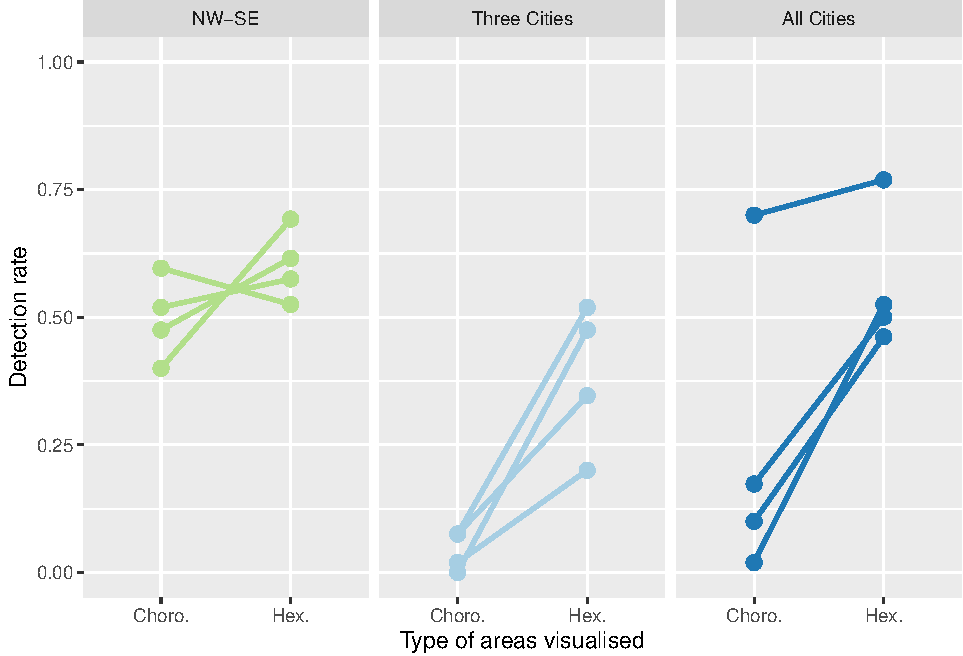
\includegraphics{paper_files/figure-latex/detection_compare-1.pdf}
\caption{Each point shows the probability of detection for the lineup
display, separated by the trend model hidden in the lineup. The points
for the same data set are linked to show the difference in the detection
rate when the same data was seen in each display. 11 of the 12 real
distribution plots were found more often in the hexagon display.}
\end{figure}

\begin{tabular}{l|l|r|r|r}
\hline
trend & type & replicate & mean & std.dev\\
\hline
NW-SE & Choropleth & 1 & 25.00 & 16.41\\
\hline
NW-SE & Choropleth & 2 & 21.12 & 15.28\\
\hline
NW-SE & Choropleth & 3 & 21.12 & 17.05\\
\hline
NW-SE & Choropleth & 4 & 21.20 & 14.52\\
\hline
NW-SE & Hexagon tiles & 1 & 19.53 & 14.56\\
\hline
NW-SE & Hexagon tiles & 2 & 21.95 & 16.42\\
\hline
NW-SE & Hexagon tiles & 3 & 22.02 & 16.12\\
\hline
NW-SE & Hexagon tiles & 4 & 18.17 & 14.51\\
\hline
three cities & Choropleth & 1 & 15.30 & 13.88\\
\hline
three cities & Choropleth & 2 & 25.22 & 14.36\\
\hline
three cities & Choropleth & 3 & 22.49 & 15.87\\
\hline
three cities & Choropleth & 4 & 18.68 & 13.74\\
\hline
three cities & Hexagon tiles & 1 & 20.37 & 17.02\\
\hline
three cities & Hexagon tiles & 2 & 19.95 & 16.59\\
\hline
three cities & Hexagon tiles & 3 & 20.02 & 17.19\\
\hline
three cities & Hexagon tiles & 4 & 18.02 & 16.93\\
\hline
all cities & Choropleth & 1 & 20.14 & 16.56\\
\hline
all cities & Choropleth & 2 & 22.75 & 14.72\\
\hline
all cities & Choropleth & 3 & 19.88 & 15.03\\
\hline
all cities & Choropleth & 4 & 19.33 & 16.15\\
\hline
all cities & Hexagon tiles & 1 & 19.83 & 15.87\\
\hline
all cities & Hexagon tiles & 2 & 16.96 & 14.65\\
\hline
all cities & Hexagon tiles & 3 & 19.21 & 15.27\\
\hline
all cities & Hexagon tiles & 4 & 20.03 & 15.11\\
\hline
\end{tabular}

A t-test shows the difference between the detection rates for the two
types of displays. The value of 0.0041593 shows that it is very unlikely
the difference is due to chance.

\hypertarget{speed}{%
\subsection{Speed}\label{speed}}

\begin{figure}
\centering
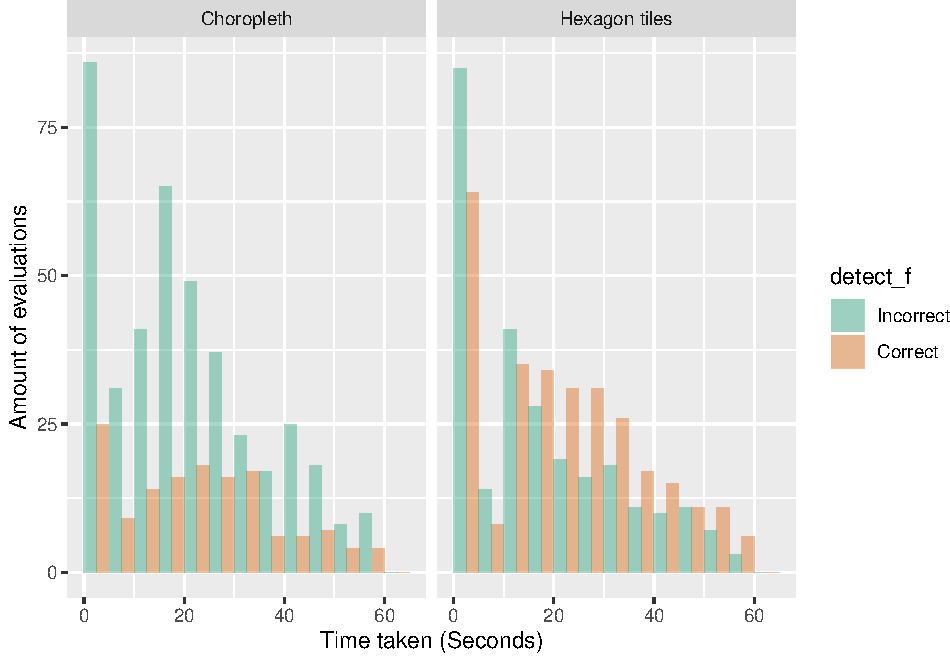
\includegraphics{paper_files/figure-latex/time-1.pdf}
\caption{The time taken to evaluate each display is broken into five
second windows. The height of the histogram bars show how many
evaulations were submitted within each time window. The distributions
for the choropleth and hexagon tile maps are very similar. Both have a
large peak at 0-5 seconds, and then a secondary peak at 10-20 seconds.
No response took over one minute.}
\end{figure}

\begin{figure}
\centering
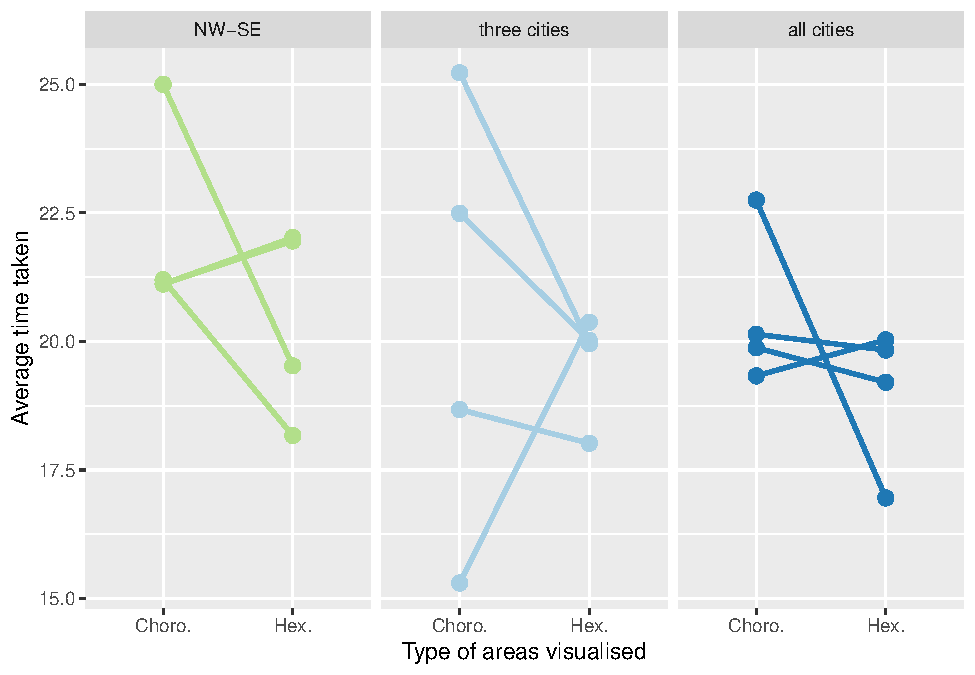
\includegraphics{paper_files/figure-latex/time_compare-1.pdf}
\caption{Each point shows the average time taken for participants to
evalute the lineup display, separated by the trend model hidden in the
lineup. The points for the same data set are linked to show the
difference in the avergae time taken when the same data was seen in each
display. There is a lot of variation in the time taken. The shortest
average time (15 seconds), and the longest average time (23 seconds)
both occured when evaluating three cities}
\end{figure}

\hypertarget{certainty}{%
\subsection{Certainty}\label{certainty}}

\begin{figure}
\centering
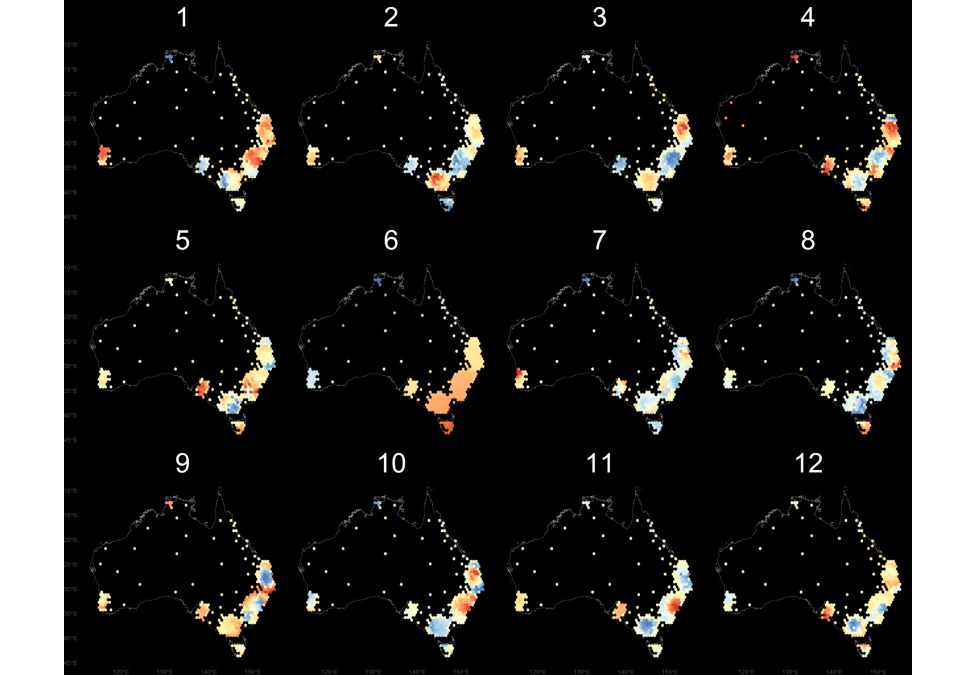
\includegraphics{paper_files/figure-latex/unnamed-chunk-1-1.pdf}
\caption{The amount of times each level of certainty was chosen by
participants when viewing hexagon tile map or choropleth displays.
Participants were more likely to choose a high certainty when
considering a Choropleth map. The default certainty of 3 was chosen most
for the Hexagon tile map displays.}
\end{figure}

Certainty levels are measured on a five point scale---they are
subjective assessments by the participant `how certain are you about
your choice?'.

\begin{figure}
\centering
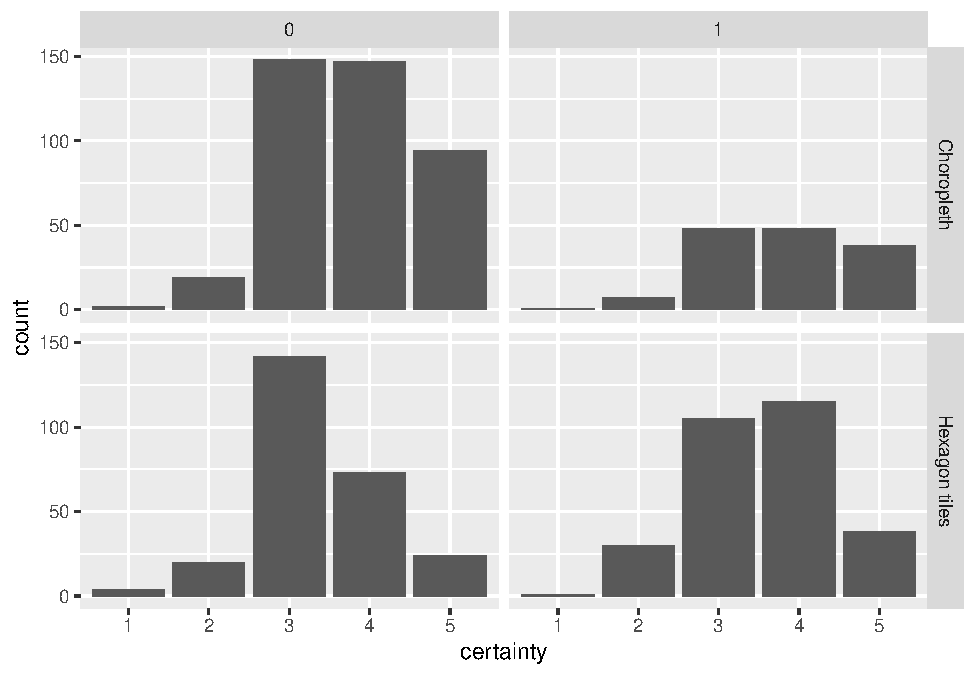
\includegraphics{paper_files/figure-latex/unnamed-chunk-2-1.pdf}
\caption{The amount of times each level of certainty was chosen by
participants. The columns shown whether a viewer correctly selected the
real trend data plot when viewing hexagon tile map or choropleth
displays.}
\end{figure}

\begin{figure}
\centering
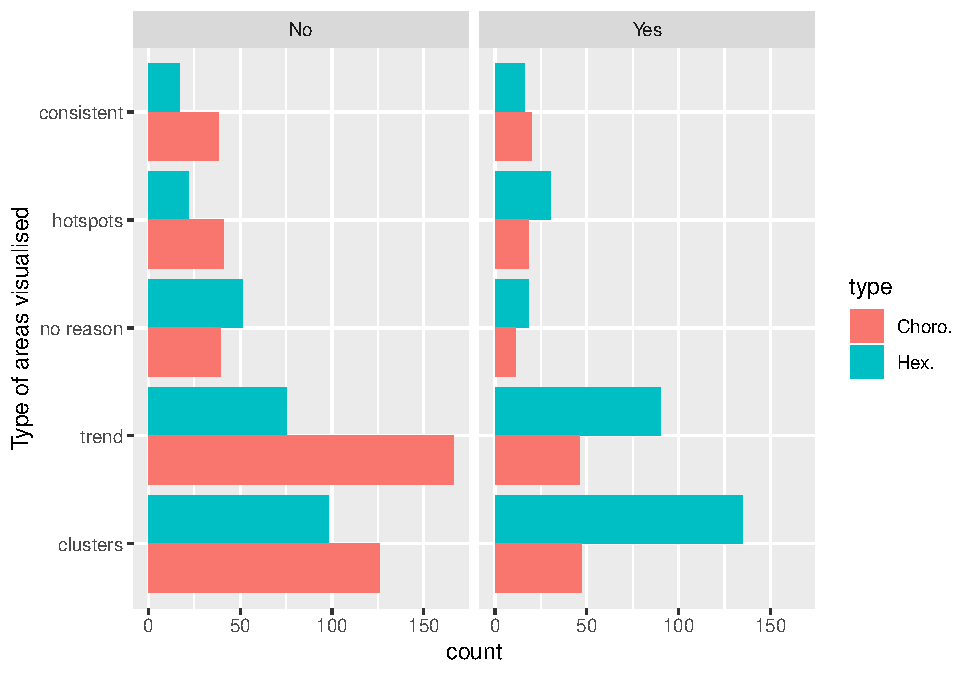
\includegraphics{paper_files/figure-latex/unnamed-chunk-3-1.pdf}
\caption{The amount of times each level of certainty was chosen by
participants. The columns shown whether a viewer correctly selected the
real trend data plot when viewing hexagon tile map or choropleth
displays. The rows show the type of the trend model added in the real
data plot. The default certainty level of 3 was chosen most frequently
when incorrect. Then shown a NW-SE or all cities trend participants felt
more certain of their correct choice.}
\end{figure}

\hypertarget{reason}{%
\subsection{Reason}\label{reason}}

\begin{figure}
\centering
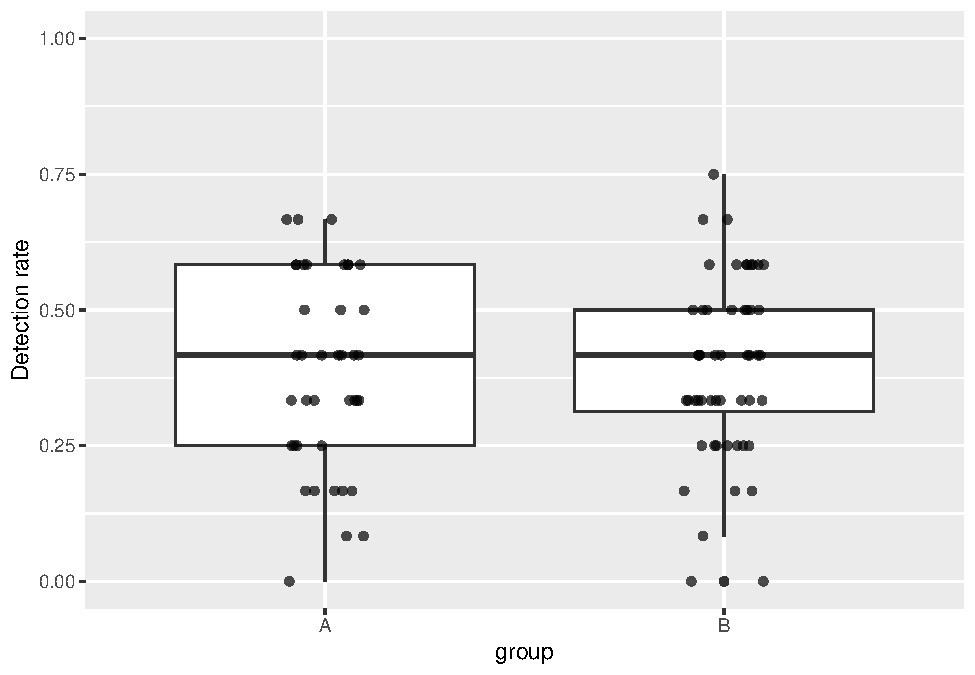
\includegraphics{paper_files/figure-latex/unnamed-chunk-4-1.pdf}
\caption{The most common reason for choice of plot when looking at each
trend model shown in Choropleth and Hexagon Tile maps. Clusters were the
most common reason when viewing a Hexagon Tile map, trend was the most
common choice for choropleth displays except for the all cities
display.}
\end{figure}

\hypertarget{contributors}{%
\subsection{Contributors}\label{contributors}}

\begin{figure}
\centering
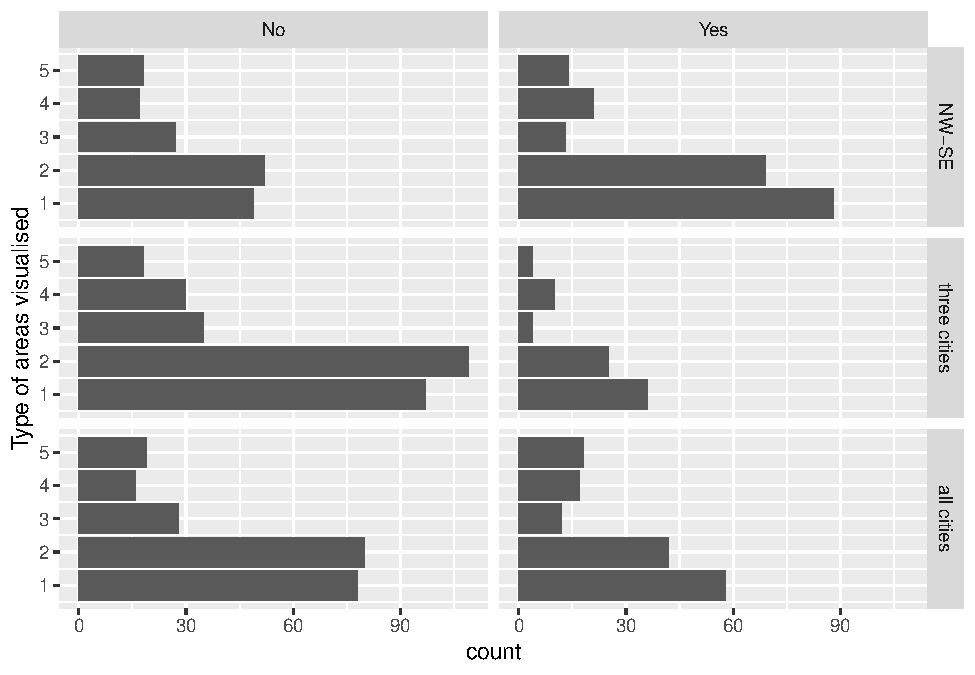
\includegraphics{paper_files/figure-latex/unnamed-chunk-5-1.pdf}
\caption{The probablity of detection acheived by the contributors in
each group is shown by the points. Group B has a larger range and a
smaller inter-quartile range. Group A and both had 3 people who did not
find any of the data maps in the displays.}
\end{figure}

\hypertarget{reason-1}{%
\subsection{Reason}\label{reason-1}}

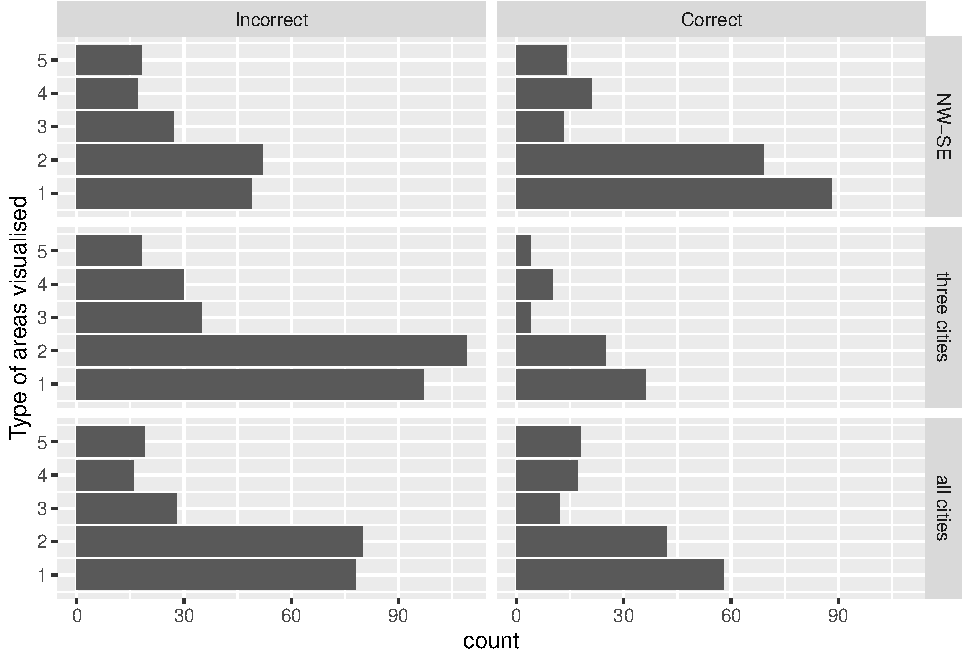
\includegraphics{paper_files/figure-latex/unnamed-chunk-6-1.pdf}

\begin{figure}
\centering
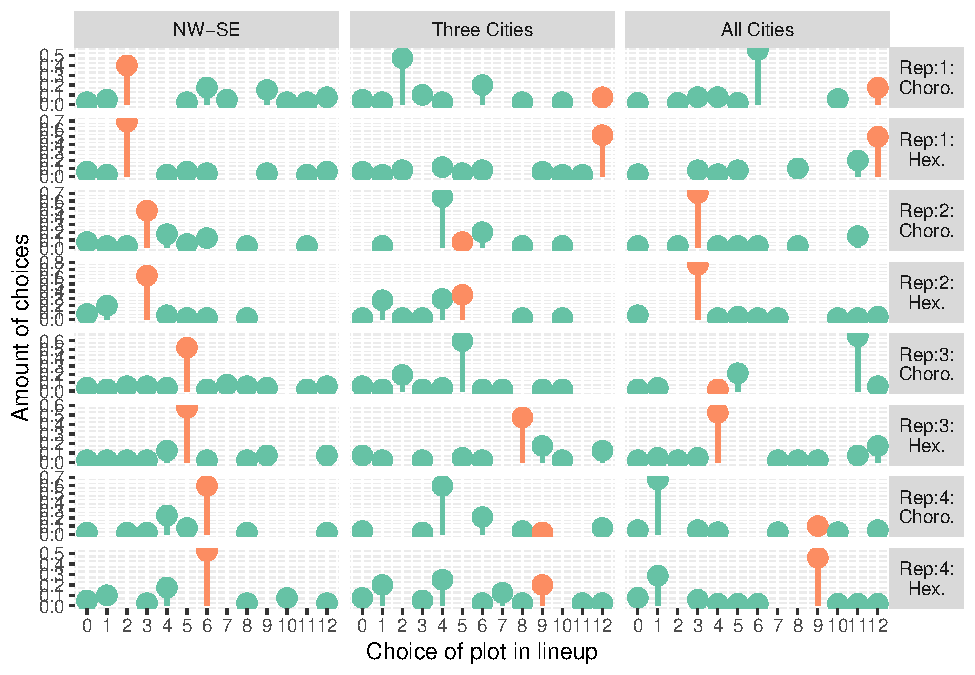
\includegraphics{paper_files/figure-latex/choices-1.pdf}
\caption{Each facet is associated with one lineup, the height of the
bars count the choices made by the participants considering each lineup.
The bars coloured with black outlines show the map which contained a
trend model, these are the correct choices. The numbers differentiate
the replicates of each trend model and type of map display. Participants
were able to select 0 to indicate they did not want to choose a map.}
\end{figure}

The choices made by participants are examined in Figure
\ref{fig:choices}. Participants were misled by the choropleth display,
but not the hexagon display for all cities displays except (2). The maps
with a North West to South East trend was chosen with much greater
frequency in all displays. All of three cities displays, except (4),
were detected in the hexagon display. All except one lineup had at least
one participant select the correct map in the lineup as shown in Figure
\ref{fig:choices}.

\hypertarget{anomolies}{%
\subsection{Anomolies}\label{anomolies}}

\hypertarget{modeling-the-difference}{%
\subsection{Modeling the difference}\label{modeling-the-difference}}

A generalized linear mixed effects model can account for each individual
participants' abilities as it includes a subject-specific random
intercept. As each participant provides results from 12 lineups.

\hypertarget{detection-rates}{%
\subsubsection{Detection Rates}\label{detection-rates}}

\begin{verbatim}
## # A tibble: 6 x 5
##   term                                estimate std.error statistic p.value
##   <chr>                                  <dbl>     <dbl>     <dbl>   <dbl>
## 1 (Intercept)                           0.0217     0.147     0.147   0.883
## 2 typeHexagon tiles                     0.420      0.211     1.99    0.047
## 3 trendthree cities                    -3.25       0.412    -7.88    0    
## 4 trendall cities                      -1.24       0.229    -5.41    0    
## 5 typeHexagon tiles:trendthree cities   2.37       0.465     5.10    0    
## 6 typeHexagon tiles:trendall cities     1.08       0.312     3.47    0.001
\end{verbatim}

\begin{verbatim}
## Analysis of Deviance Table
## 
## Model: binomial, link: logit
## 
## Response: detect_f
## 
## Terms added sequentially (first to last)
## 
## 
##            Df Deviance Resid. Df Resid. Dev  Pr(>Chi)    
## NULL                        1103     1477.0              
## type        1   83.526      1102     1393.5 < 2.2e-16 ***
## trend       2  101.699      1100     1291.8 < 2.2e-16 ***
## type:trend  2   35.517      1098     1256.2 1.939e-08 ***
## ---
## Signif. codes:  0 '***' 0.001 '**' 0.01 '*' 0.05 '.' 0.1 ' ' 1
\end{verbatim}

\begin{verbatim}
##            
##             Incorrect Correct
##   Incorrect       431     121
##   Correct         242     310
\end{verbatim}

\begin{verbatim}
## # A tibble: 1 x 6
##   sigma logLik   AIC   BIC deviance df.residual
##   <dbl>  <dbl> <dbl> <dbl>    <dbl>       <int>
## 1 0.430  -675. 1367. 1407.    1321.        1096
\end{verbatim}

\begin{verbatim}
## # A tibble: 8 x 5
##   term                                estimate std.error statistic group      
##   <chr>                                  <dbl>     <dbl>     <dbl> <chr>      
## 1 (Intercept)                            0.505    0.0340     14.9  fixed      
## 2 typeHexagon tiles                      0.103    0.0448      2.31 fixed      
## 3 trendthree cities                     -0.467    0.0448    -10.4  fixed      
## 4 trendall cities                       -0.277    0.0448     -6.19 fixed      
## 5 typeHexagon tiles:trendthree cities    0.250    0.0633      3.95 fixed      
## 6 typeHexagon tiles:trendall cities      0.239    0.0633      3.77 fixed      
## 7 sd_(Intercept).contributor             0.118   NA          NA    contributor
## 8 sd_Observation.Residual                0.430   NA          NA    Residual
\end{verbatim}

\begin{verbatim}
##            
##             Incorrect Correct
##   Incorrect        49       1
##   Correct         624     430
\end{verbatim}

For a base model of Choropleth map, using a NW-SE trend model. The
detection rate for Hexagon tile maps using a NW-SE trend model changes
the log odds of the detection by 0.42.

\hypertarget{certainty-1}{%
\subsubsection{Certainty}\label{certainty-1}}

\begin{verbatim}
## Linear mixed model fit by REML ['lmerMod']
## Formula: detect ~ type * trend + (1 | contributor)
##    Data: d
## REML criterion at convergence: 1350.719
## Random effects:
##  Groups      Name        Std.Dev.
##  contributor (Intercept) 0.1179  
##  Residual                0.4296  
## Number of obs: 1104, groups:  contributor, 92
## Fixed Effects:
##                         (Intercept)                    typeHexagon tiles  
##                              0.5054                               0.1033  
##                   trendthree cities                      trendall cities  
##                             -0.4674                              -0.2772  
## typeHexagon tiles:trendthree cities    typeHexagon tiles:trendall cities  
##                              0.2500                               0.2391
\end{verbatim}

\hypertarget{discussion}{%
\section{Discussion}\label{discussion}}

\hypertarget{conclusion}{%
\section{Conclusion}\label{conclusion}}

how do the results found generalise to other work - Not just for Aus
(Canada new Zealand could also use this effective display)

\begin{itemize}
\tightlist
\item
  For USA alternative methods can also be helpful
\end{itemize}

\hypertarget{supplementary-materials}{%
\section{Supplementary Materials}\label{supplementary-materials}}

\hypertarget{training}{%
\subsection{Training}\label{training}}

\hypertarget{survey-application}{%
\subsection{Survey application}\label{survey-application}}

\hypertarget{subject-specific-anomolies-0-detection}{%
\subsection{Subject specific anomolies (0\%
detection)}\label{subject-specific-anomolies-0-detection}}

\hypertarget{acknowledgment}{%
\section{Acknowledgment}\label{acknowledgment}}

The authors would like to thank\ldots{}

Ethics approval for the online survey was granted by QUT's Ethics
Committee (Ethics Application Number: 1900000991). All applicants
provided informed consent in line with QUT regulations prior to
participating in this research.

\hypertarget{bibliography-styles}{%
\section{Bibliography styles}\label{bibliography-styles}}

\newpage

\hypertarget{references}{%
\section{References}\label{references}}

\hypertarget{refs}{}
\leavevmode\hypertarget{ref-abs2016}{}%
``Australian Statistical Geography Standard (ASGS).'' 2018.
\emph{Australian Bureau of Statistics}. Australian Government.
\url{\%7Bhttps://www.abs.gov.au/websitedbs/D3310114.nsf/home/Australian\%20\%20\%20Statistical\%20Geography\%20Standard\%20(ASGS)\%7D}.

\leavevmode\hypertarget{ref-lme4}{}%
Bates, Douglas, Martin Mächler, Ben Bolker, and Steve Walker. 2015.
``Fitting Linear Mixed-Effects Models Using lme4.'' \emph{Journal of
Statistical Software} 67 (1): 1--48.
\url{https://doi.org/10.18637/jss.v067.i01}.

\leavevmode\hypertarget{ref-sheets}{}%
Bryan, Jennifer, and Joanna Zhao. 2018. \emph{Googlesheets: Manage
Google Spreadsheets from R}.
\url{https://CRAN.R-project.org/package=googlesheets}.

\leavevmode\hypertarget{ref-SIEDAMD}{}%
Buja, Andreas, Dianne Cook, Heike Hofmann, Michael Lawrence, Eun-Kyung
Lee, Deborah F. Swayne, and Hadley Wlckham. 2009. ``Statistical
Inference for Exploratory Data Analysis and Model Diagnostics.''
\emph{Philosophical Transactions: Mathematical, Physical and Engineering
Sciences} 367 (1906): 4361--83.
\url{http://www.jstor.org/stable/40485732}.

\leavevmode\hypertarget{ref-VVSIALM}{}%
Majumder, Mahbubul, Heike Hofmann, and Dianne Cook. 2013. ``Validation
of Visual Statistical Inference, Applied to Linear Models.''
\emph{Journal of the American Statistical Association} 108 (503):
942--56. \url{https://doi.org/10.1080/01621459.2013.808157}.

\leavevmode\hypertarget{ref-RCore}{}%
R Core Team. 2019. \emph{R: A Language and Environment for Statistical
Computing}. Vienna, Austria: R Foundation for Statistical Computing.
\url{https://www.R-project.org/}.

\end{document}


